\documentclass[12pt,a4paper,final,titlepage,twoside]{article}
\usepackage{MLABdoc}
\fancyhead[L]{{\huge RPS01A}}
\fancyfoot[RE,LO]{\today\hspace{1pt}|  | mlab.cz}

\includeonly{RPS01A.cs.title, RPS01A.cs.assembly}

\begin{document}
%vytvori uvodni stranku
\uvod
% nazev modulu
{RPS01A}
% kratky popis
{Magnetické rotační čidlo absolutní pozice}
%autor/i
{}
%obrazek
{../..//doc/img/RPS01A_top_big.jpg}
%abstrakt
{Bezkontaktní magnetické čidlo pozice. K měření je pouze potřeba dvoupólový magnet rotující nad středem čipu. Změřená pozice pak může být vyčtena digitálním rozhraním.}
%tabulka
{ }
%obrazek QR kodu
{../../doc/img/RPS01A_QRcode.png}


\section{Popis konstrukce}
Modul obsahuje úchytné šroubky ve všech rozích v rozteči MLAB (10.16mm). Při potřebě šetřit místem je možné odstřihnutí části PCB se dvěma šrouby.
\subsection{Zapojení}
%naimportuje schema 
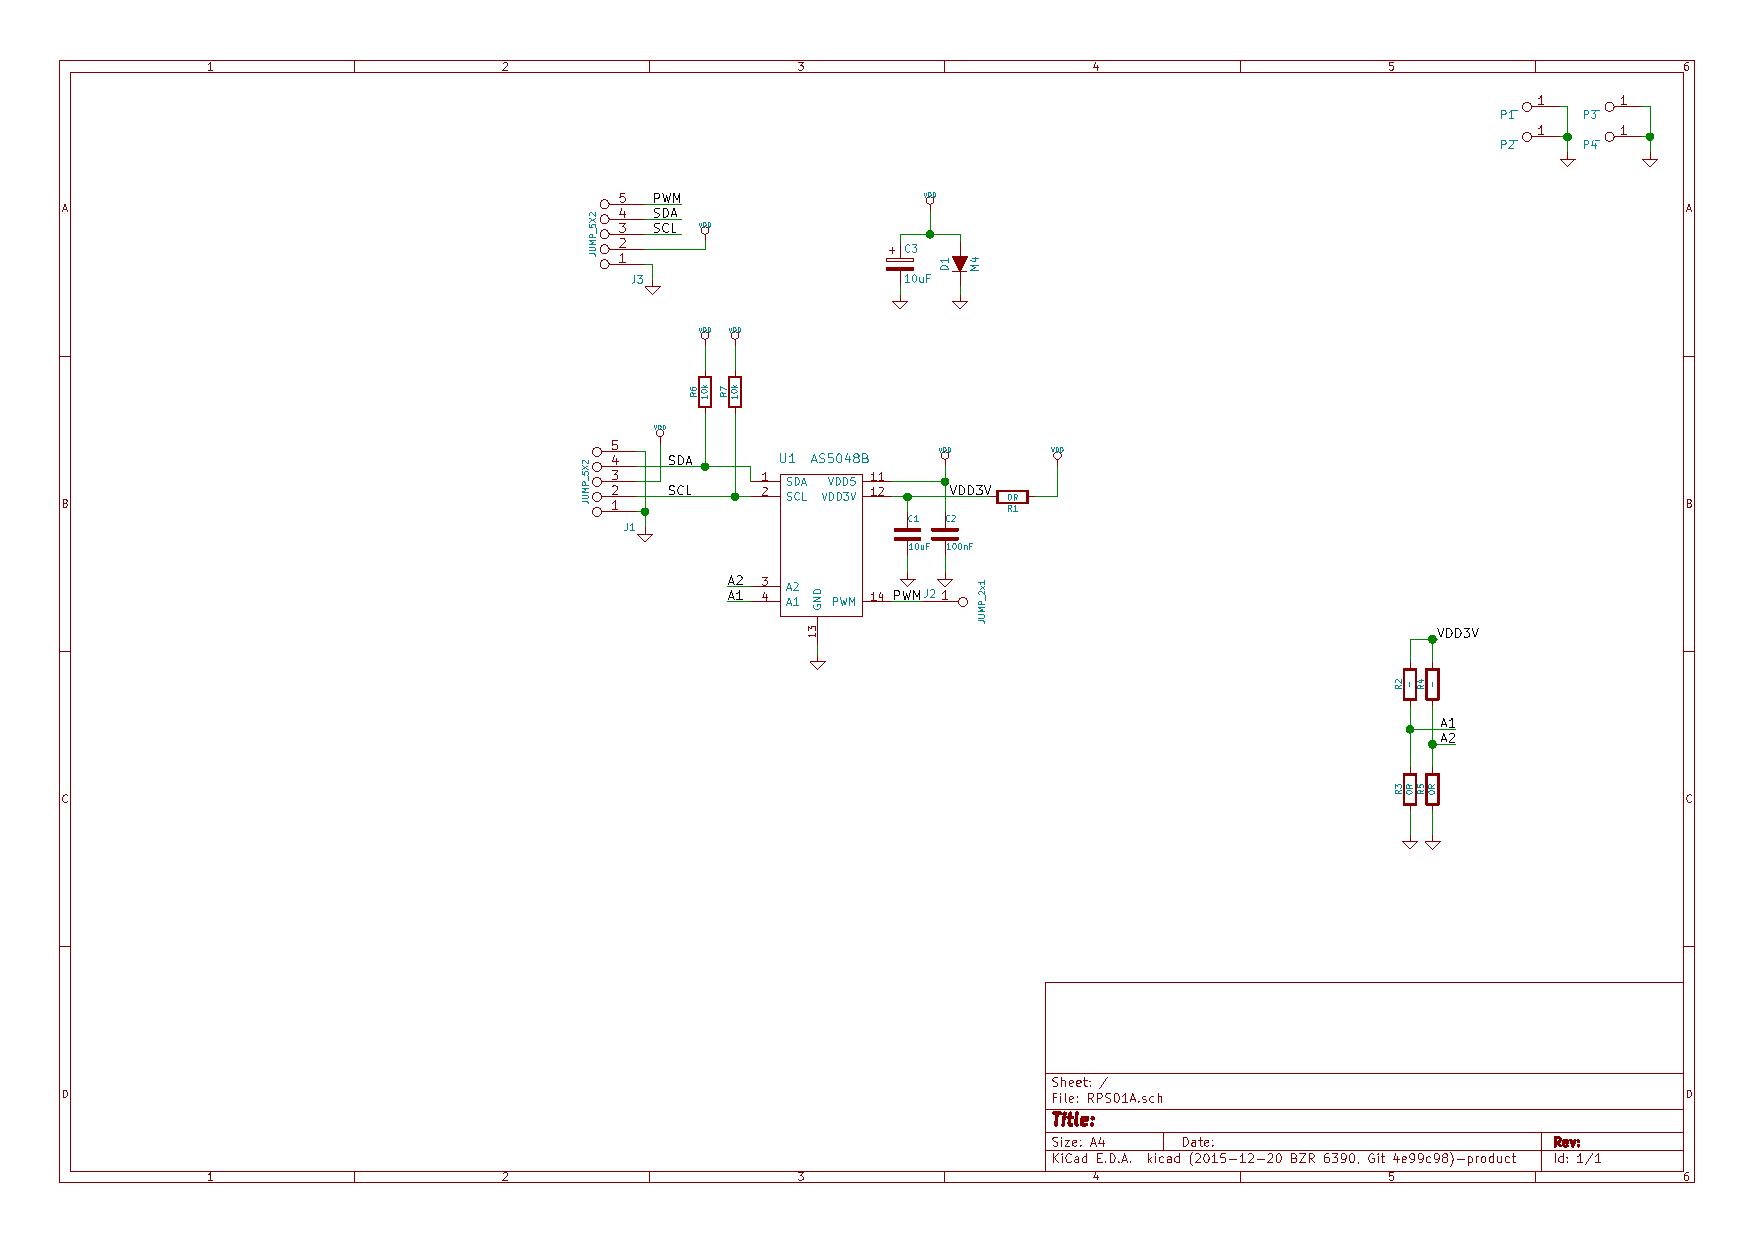
\includepdf[angle=90]{../../hw/sch_pcb/RPS01A.pdf}

\subsection{Odrušení}

\subsection{Mechanická konstrukce}

\section{Výroba a testování}

% totot naimportuje cast, kde jsou osazováky a BOM tabulka
\subsection{Osazení}


\begin{figure}[ht!]
	\centering
	\includegraphics[scale=2]{../../hw/CAM_PROFI/RPS01A-top_cropped.pdf}
	\qquad
	\includegraphics[scale=2]{../../hw/CAM_PROFI/RPS01A-bottom_cropped.pdf}
\end{figure}

\begin{center}
  \begin{tabular}{ | l | l | l | l |}
    \hline
    Označení & Hodnota, typ & Pouzdro & Počet \\ \hline
    \hline
			C2 & 100nF &  & 1\\ \hline
			C1 & 10uF &  & 1\\ \hline
			D1 & M4 &  & 1\\ \hline
			U1 & AS5048B &  & 1\\ \hline
			J2 & JUMP\_2x1 &  & 1\\ \hline
			R1, R3, R5 & 0R &  & 3\\ \hline
			R6, R7 & 10k &  & 2\\ \hline
			R4, R2 & - &  & 2\\ \hline
			J1, J3 & JUMP\_5X2 &  & 2\\ \hline
			C3 & 10uF &  & 1\\ \hline
			P1, P2, P3, P4 & \_ &  & 4\\ \hline
	
  \end{tabular}
\end{center}
\subsection{Oživení}
Vzorový program je napsán v programu pyMLAB.

\end{document}